\documentclass[12pt,a4paper]{article}

%% 使用ctex规定中文样式
\usepackage{ctex}
%% 使用xeCJK, 設定中英文的字型
\usepackage{xeCJK}
%% 设置缺省英文字体
\setmainfont{Times New Roman}
\setmonofont{Courier New}
%% 设置缺省中文字体
\setCJKmainfont[BoldFont=STXinwei]{DFKai-SB} %標楷體,华文新魏
%\setCJKmainfont[BoldFont=SimHei]{SimSun} %宋体,黑体
\setCJKmonofont{SimSun}

\usepackage{amsmath} %公式
\usepackage{graphicx} %处理图形
\usepackage{subfig} %子图
\usepackage{booktabs} %美化表格

\renewcommand\figurename{图}
\renewcommand\tablename{表}

\title{标题}
\author{
	作者 \thanks{学号,单位,邮箱} %\thanks 中不能使用\\
}
\date{\today}

\begin{document}
\maketitle

\section{章节}
\subsection{小章节}
\subsubsection{子章节}

\noindent 强制无缩进 


\section{公式}
单行公式
\begin{equation}
f(x) = \frac{1}{\sigma} \phi\left(\frac{x-\mu}{\sigma}\right)
\end{equation}

多行公式(居中对齐)
\begin{gather*} 
2x - 5y =  8 \\ 
3x^2 + 9y =  3a + c
\end{gather*}

多行公式(指定对齐)
\begin{align} %不要用eqnarray环境
& r = R/(R+G+B) & \nonumber \\
& b = B/(R+G+B) & \text{公式内文字} % &用于竖直对齐
\end{align}

%% more, go to: https://en.wikibooks.org/wiki/LaTeX/Advanced_Mathematics
%% or: http://www.sharelatex.com/learn/Aligning_equations_with_amsmath

\section{列表}
无序:
\begin{itemize}
\item  C++
\item  Java
\item  HTML
\end{itemize}

有序:
\begin{enumerate}
\item  C++
\item  Java
\item  HTML
\end{enumerate}

描述:
\begin{description}
\item{C++:}  一种编程语言
\item{Java:}  另一种编程语言
\item{HTML:}  一种标记语言
\end{description}

\section{表格}
普通表(\ref{tab:a}):
\begin{table}[htbp]
\caption{浮动环境中的三线表}
\label{tab:a}
\centering
\begin{tabular}{l|c|r} % |是竖直分隔,lcr是对齐方式
\hline %水平分隔
操作系统  &  发行版  &  编辑器  \\
\hline
Windows  &  MikTeX  &  TeXnicCenter  \\
Unix/Linux  &  TeX  Live  &  Emacs  \\
Mac  OS  &  MacTeX  &  TeXShop  \\
\hline
\end{tabular}
\end{table}

网络书籍常用表(\ref{tab:b}):
\begin{table}[htbp]
\caption{另外的三线表}
\label{tab:b}
\centering
\begin{tabular}{lll}
\toprule
操作系统  &  发行版  &  编辑器  \\
\midrule
Windows  &  MikTeX  &  TeXnicCenter  \\
Unix/Linux  &  TeX  Live  &  Emacs  \\
Mac  OS  &  MacTeX  &  TeXShop  \\
\bottomrule
\end{tabular}
\end{table}

%% https://en.wikibooks.org/wiki/LaTeX/Tables

\section{图片}
并列子图,引用图(\ref{fig:a})。
\begin{figure}[htbp!]
\centerline{
	\subfloat[Original]{
		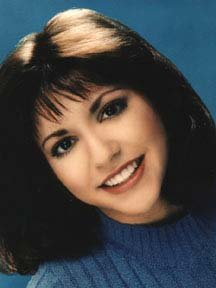
\includegraphics[width=0.3\textwidth]{./res/s1.jpg}
	}
	\hfil
	\subfloat[Skin-likelihood]{
		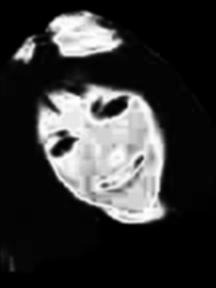
\includegraphics[width=0.3\textwidth]{./res/s2.jpg}
	}
	\hfil
	\subfloat[Skin-segmented]{
		
\includegraphics[width=0.3\textwidth]{./res/s3.jpg}
	}
}
\caption{Image processing sequences for graduation image.}
\label{fig:a}
\end{figure}

%% https://en.wikibooks.org/wiki/LaTeX/Floats,_Figures_and_Captions




\end{document} 

